\documentclass[english,,man]{apa6}
\usepackage{lmodern}
\usepackage{amssymb,amsmath}
\usepackage{ifxetex,ifluatex}
\usepackage{fixltx2e} % provides \textsubscript
\ifnum 0\ifxetex 1\fi\ifluatex 1\fi=0 % if pdftex
  \usepackage[T1]{fontenc}
  \usepackage[utf8]{inputenc}
\else % if luatex or xelatex
  \ifxetex
    \usepackage{mathspec}
  \else
    \usepackage{fontspec}
  \fi
  \defaultfontfeatures{Ligatures=TeX,Scale=MatchLowercase}
\fi
% use upquote if available, for straight quotes in verbatim environments
\IfFileExists{upquote.sty}{\usepackage{upquote}}{}
% use microtype if available
\IfFileExists{microtype.sty}{%
\usepackage{microtype}
\UseMicrotypeSet[protrusion]{basicmath} % disable protrusion for tt fonts
}{}
\usepackage{hyperref}
\hypersetup{unicode=true,
            pdftitle={Process Cookbook},
            pdfauthor={\ldots{}},
            pdfkeywords={\ldots{}.},
            pdfborder={0 0 0},
            breaklinks=true}
\urlstyle{same}  % don't use monospace font for urls
\ifnum 0\ifxetex 1\fi\ifluatex 1\fi=0 % if pdftex
  \usepackage[shorthands=off,main=english]{babel}
\else
  \usepackage{polyglossia}
  \setmainlanguage[]{english}
\fi
\usepackage{color}
\usepackage{fancyvrb}
\newcommand{\VerbBar}{|}
\newcommand{\VERB}{\Verb[commandchars=\\\{\}]}
\DefineVerbatimEnvironment{Highlighting}{Verbatim}{commandchars=\\\{\}}
% Add ',fontsize=\small' for more characters per line
\usepackage{framed}
\definecolor{shadecolor}{RGB}{248,248,248}
\newenvironment{Shaded}{\begin{snugshade}}{\end{snugshade}}
\newcommand{\AlertTok}[1]{\textcolor[rgb]{0.94,0.16,0.16}{#1}}
\newcommand{\AnnotationTok}[1]{\textcolor[rgb]{0.56,0.35,0.01}{\textbf{\textit{#1}}}}
\newcommand{\AttributeTok}[1]{\textcolor[rgb]{0.77,0.63,0.00}{#1}}
\newcommand{\BaseNTok}[1]{\textcolor[rgb]{0.00,0.00,0.81}{#1}}
\newcommand{\BuiltInTok}[1]{#1}
\newcommand{\CharTok}[1]{\textcolor[rgb]{0.31,0.60,0.02}{#1}}
\newcommand{\CommentTok}[1]{\textcolor[rgb]{0.56,0.35,0.01}{\textit{#1}}}
\newcommand{\CommentVarTok}[1]{\textcolor[rgb]{0.56,0.35,0.01}{\textbf{\textit{#1}}}}
\newcommand{\ConstantTok}[1]{\textcolor[rgb]{0.00,0.00,0.00}{#1}}
\newcommand{\ControlFlowTok}[1]{\textcolor[rgb]{0.13,0.29,0.53}{\textbf{#1}}}
\newcommand{\DataTypeTok}[1]{\textcolor[rgb]{0.13,0.29,0.53}{#1}}
\newcommand{\DecValTok}[1]{\textcolor[rgb]{0.00,0.00,0.81}{#1}}
\newcommand{\DocumentationTok}[1]{\textcolor[rgb]{0.56,0.35,0.01}{\textbf{\textit{#1}}}}
\newcommand{\ErrorTok}[1]{\textcolor[rgb]{0.64,0.00,0.00}{\textbf{#1}}}
\newcommand{\ExtensionTok}[1]{#1}
\newcommand{\FloatTok}[1]{\textcolor[rgb]{0.00,0.00,0.81}{#1}}
\newcommand{\FunctionTok}[1]{\textcolor[rgb]{0.00,0.00,0.00}{#1}}
\newcommand{\ImportTok}[1]{#1}
\newcommand{\InformationTok}[1]{\textcolor[rgb]{0.56,0.35,0.01}{\textbf{\textit{#1}}}}
\newcommand{\KeywordTok}[1]{\textcolor[rgb]{0.13,0.29,0.53}{\textbf{#1}}}
\newcommand{\NormalTok}[1]{#1}
\newcommand{\OperatorTok}[1]{\textcolor[rgb]{0.81,0.36,0.00}{\textbf{#1}}}
\newcommand{\OtherTok}[1]{\textcolor[rgb]{0.56,0.35,0.01}{#1}}
\newcommand{\PreprocessorTok}[1]{\textcolor[rgb]{0.56,0.35,0.01}{\textit{#1}}}
\newcommand{\RegionMarkerTok}[1]{#1}
\newcommand{\SpecialCharTok}[1]{\textcolor[rgb]{0.00,0.00,0.00}{#1}}
\newcommand{\SpecialStringTok}[1]{\textcolor[rgb]{0.31,0.60,0.02}{#1}}
\newcommand{\StringTok}[1]{\textcolor[rgb]{0.31,0.60,0.02}{#1}}
\newcommand{\VariableTok}[1]{\textcolor[rgb]{0.00,0.00,0.00}{#1}}
\newcommand{\VerbatimStringTok}[1]{\textcolor[rgb]{0.31,0.60,0.02}{#1}}
\newcommand{\WarningTok}[1]{\textcolor[rgb]{0.56,0.35,0.01}{\textbf{\textit{#1}}}}
\usepackage{graphicx,grffile}
\makeatletter
\def\maxwidth{\ifdim\Gin@nat@width>\linewidth\linewidth\else\Gin@nat@width\fi}
\def\maxheight{\ifdim\Gin@nat@height>\textheight\textheight\else\Gin@nat@height\fi}
\makeatother
% Scale images if necessary, so that they will not overflow the page
% margins by default, and it is still possible to overwrite the defaults
% using explicit options in \includegraphics[width, height, ...]{}
\setkeys{Gin}{width=\maxwidth,height=\maxheight,keepaspectratio}
\IfFileExists{parskip.sty}{%
\usepackage{parskip}
}{% else
\setlength{\parindent}{0pt}
\setlength{\parskip}{6pt plus 2pt minus 1pt}
}
\setlength{\emergencystretch}{3em}  % prevent overfull lines
\providecommand{\tightlist}{%
  \setlength{\itemsep}{0pt}\setlength{\parskip}{0pt}}
\setcounter{secnumdepth}{0}
% Redefines (sub)paragraphs to behave more like sections
\ifx\paragraph\undefined\else
\let\oldparagraph\paragraph
\renewcommand{\paragraph}[1]{\oldparagraph{#1}\mbox{}}
\fi
\ifx\subparagraph\undefined\else
\let\oldsubparagraph\subparagraph
\renewcommand{\subparagraph}[1]{\oldsubparagraph{#1}\mbox{}}
\fi

%%% Use protect on footnotes to avoid problems with footnotes in titles
\let\rmarkdownfootnote\footnote%
\def\footnote{\protect\rmarkdownfootnote}


  \title{Process Cookbook}
    \author{\ldots{}\textsuperscript{1}}
    \date{}
  
\shorttitle{PROCESS INFERENCES}
\authornote{....


Correspondence concerning this article should be addressed to ..., .... E-mail: ...}
\affiliation{
\vspace{0.5cm}
\textsuperscript{1} ...}
\abstract{Begin here...
}
\keywords{....\newline\indent Word count: 95}
\usepackage{csquotes}
\usepackage{upgreek}
\captionsetup{font=singlespacing,justification=justified}

\usepackage{longtable}
\usepackage{lscape}
\usepackage{multirow}
\usepackage{tabularx}
\usepackage[flushleft]{threeparttable}
\usepackage{threeparttablex}

\newenvironment{lltable}{\begin{landscape}\begin{center}\begin{ThreePartTable}}{\end{ThreePartTable}\end{center}\end{landscape}}

\makeatletter
\newcommand\LastLTentrywidth{1em}
\newlength\longtablewidth
\setlength{\longtablewidth}{1in}
\newcommand{\getlongtablewidth}{\begingroup \ifcsname LT@\roman{LT@tables}\endcsname \global\longtablewidth=0pt \renewcommand{\LT@entry}[2]{\global\advance\longtablewidth by ##2\relax\gdef\LastLTentrywidth{##2}}\@nameuse{LT@\roman{LT@tables}} \fi \endgroup}


\DeclareDelayedFloatFlavor{ThreePartTable}{table}
\DeclareDelayedFloatFlavor{lltable}{table}
\DeclareDelayedFloatFlavor*{longtable}{table}
\makeatletter
\renewcommand{\efloat@iwrite}[1]{\immediate\expandafter\protected@write\csname efloat@post#1\endcsname{}}
\makeatother
\usepackage{lineno}

\linenumbers

\usepackage{amsthm}
\newtheorem{theorem}{Theorem}[section]
\newtheorem{lemma}{Lemma}[section]
\theoremstyle{definition}
\newtheorem{definition}{Definition}[section]
\newtheorem{corollary}{Corollary}[section]
\newtheorem{proposition}{Proposition}[section]
\theoremstyle{definition}
\newtheorem{example}{Example}[section]
\theoremstyle{definition}
\newtheorem{exercise}{Exercise}[section]
\theoremstyle{remark}
\newtheorem*{remark}{Remark}
\newtheorem*{solution}{Solution}
\begin{document}
\maketitle

\hypertarget{hook-thoughts}{%
\section{Hook thoughts}\label{hook-thoughts}}

\hypertarget{hook-from-last-meeting}{%
\subsection{Hook from last meeting}\label{hook-from-last-meeting}}

\hypertarget{a-it-is-confusing-and-we-would-like-to-organize-argument}{%
\subsubsection{\texorpdfstring{A \enquote{it is confusing and we would
like to organize}
argument}{A ``it is confusing and we would like to organize'' argument}}\label{a-it-is-confusing-and-we-would-like-to-organize-argument}}

\begin{itemize}
\tightlist
\item
  New researchers are increasingly asked to collect longitudinal data.
  We care about longitudinal data.
\item
  The longitudinal literature appears more confusing than it is because
  people propose different hypotheses, use different models, and make
  different inferences.
\item
  We organize and discuss the similarities.
\end{itemize}

\hypertarget{bliese-paper-hook}{%
\subsection{Bliese paper hook}\label{bliese-paper-hook}}

\hypertarget{a-this-other-technique-can-augment-what-you-are-doing-argument}{%
\subsubsection{\texorpdfstring{A \enquote{this other technique can
augment what you are doing}
argument}{A ``this other technique can augment what you are doing'' argument}}\label{a-this-other-technique-can-augment-what-you-are-doing-argument}}

\begin{itemize}
\tightlist
\item
  We increasingly have access to longitudinal data that contain
  discontinuities.
\item
  Examples.
\item
  These studies use a variety of techniques to understand discontinuous
  patterns, but we believe that discontinuous growth models can augment
  existing techniques\ldots{}
\item
  Practical advice is spread across numerous sources and is basic -- we
  review.
\end{itemize}

\hypertarget{aguinis-paper-hook}{%
\subsection{Aguinis paper hook}\label{aguinis-paper-hook}}

\hypertarget{a-this-literature-is-technical-and-mathy-not-accessible-to-org-researchers-argument.}{%
\subsubsection{\texorpdfstring{A \enquote{this literature is technical
and mathy, not accessible to org researchers}
argument.}{A ``this literature is technical and mathy, not accessible to org researchers'' argument.}}\label{a-this-literature-is-technical-and-mathy-not-accessible-to-org-researchers-argument.}}

\begin{itemize}
\tightlist
\item
  We care about A or B.
\item
  There is a large technical literature on A or B.
\item
  Much of this work is not easily accessible to researchers with the
  usual methodological and statistical background obtained from doctoral
  level training in management.
\item
  We provide recommendations.
\end{itemize}

\hypertarget{thoughts-from-last-meeting}{%
\subsection{Thoughts from last
meeting}\label{thoughts-from-last-meeting}}

\hypertarget{a-no-argument-but-describing-paper}{%
\subsubsection{A no argument but describing
paper}\label{a-no-argument-but-describing-paper}}

\begin{itemize}
\tightlist
\item
  We care about longitudinal data
\item
  Our literature now contains a lot of cool examples and inferences
\item
  We are going to describe them
\item
  This paper is for newcomers who want some examples and for
  longitudinal modelers who want other options to augment what they are
  doing
\end{itemize}

Organizational researchers are increasingly interested in longitudinal
data structures. These data align with the processes we study, which
\enquote{are not static but instead develop, change, and evolve over
time} (Pitariu \& Ployhart, p.~405) or are \enquote{sequences of events
that play out within each person's stream of experience} (Beal, 2015,
p.~5). If researchers can collect longitudinal data, they are then in a
better position to understand patterns over time. Bell and Kozlowski
(2003), for example, state that \enquote{longitudinal
designs\ldots{}will be far more revealing of the team phenomeon under
investigation} (p.~59). Similarly -- in their review of emotional labor
-- Grandey and Gabriel (2015) suggest that future researchers may be
much better equipped to demonstrate emotion regulation patters
\enquote{with longitudinal methods} (p.~329). Not only do longitudinal
data collections help researchers observe relationships over time, many
argue that doing so helps improve our theories. For instance, Pitariu
and Ployhart (2010) suggest that collecting longitudinal data, observing
change, and testing dynamic models \enquote{stimulates greater
refinement in our existing theories} (p.~411), and Grandey and Gabriel
(2015) urge for greater theoretical development of emotions by studying
their \enquote{reciprocal and unfolding\ldots{}processes\ldots{}through
momentary assessments or lagged effects} (p.~322). These quotes reveal
our field's emphasis on collecting longitudinal data to sufficiently
observe a process and build better theory.

A greater emphasis on longitudinal data is also apparent in our
empirical literature, where collecting repeated measures is now common.
For instance, Jones et al. (2016) observed the work attitudes of
pregnant women in their second trimester every week until they gave
birth. ({\textbf{???}}) assessed job satisfaction across three time
points that were each separated by six weeks. Matthews, Wayne, and Ford
(2014) studied work-family conflict across several months. Meier and
Spector (2013) examined counterproductive work behavior over five waves.
Hardy, Day, and Steele (2018) investigated self-regulation over 20 lab
trials. Gabriel, Diefendorff, Chandler, Moran, and Greguras (2014)
measured fit and affect five times per day for 10 consecutive work days.
Finally, Johnson, Lanaj, and Barnes (2014) observed justice behavior and
resource depletion across 10 consecutive workdays.

Armed with repeated observations, these studies then explore a variety
of interesting inferences. Hardy et al. (2018) propose and find support
for growth trends in self-regulation, metacognition, and performance.
Jones et al. (2016) conclude that concealing behaviors among pregnant
women lead to greater subsequent physical health. Johnson et al. (2014)
establish that \enquote{justice is dynamic: The frequency of actors'
justice behaviors varies day to day} (p.~10), and these daily
fluctuations predict daily changes in depletion. Finally, Meier and
Spector (2013) suggest that the effects of work stressors on
counterproductive work behaviors are not substantially different across
different time lags.

Moreover, we find different types of sophisticated modeling strategies
throughout. Meier and Spector (2013) present a sequence of path models
that test increasingly longer time lags. Hardy et al. (2018) and Jones
et al. (2016) employ bivariate cross-lagged latent growth curves, an
approach similar to the latent change model used by ({\textbf{???}}). We
also find complex hierarchical linear models in various event-sampling
studies (e.g., {\textbf{???}}; Rosen, Koopman, Gabriel, \& Johnson,
2016).

In summary, our increasing theoretical emphasis on longitudinal data and
its growing prevalence in our empirical literature has led to many
interesting inferences and model applications. Researchers are beginning
to propose hypotheses with lags and examine the reciprocal nature
between two or more variables. Studies now commonly make inferences
about change, growth, and dynamics. And sophisticated models, such as
multi-level and latent growth curves, make their appearance in almost
every longitudinal study.

We want to bring attention to this new and exciting literature.
Specifically, in this paper we describe some of the common inferences
and models researchers employ with longitudinal data. Somtimes these
studies appear unrelated due to the different language used among
various content or statistical modeling areas -- but we believe our
discussion will reveal some of their covert similarities. We discuss the
inferences, identify literature examples and hypotheses that are
consistent with each, point to various models being used to support
them, provide the code necessary to both estimate and understand what
the models are doing, and unpack some of the strengths and weaknesses of
each approach. Our paper is meant for two audiences. First, we believe
this summary will help any newcomers who want to make inferences with
their longitudinal data but are unaware of what types of inferences and
models are available. Second, this paper is meant to show seasoned
researchers other possibilities -- other inferences and models that may
augment how they currently approach longitudinal data.

Below, we discuss four common inferences researchers make with
longitudinal data: relationships over time, growth, change, and
dynamics. These do not represent every possible domain we can explore
with longitudinal data, but they do cover a large portion of the
techniques currently employed in our literature. We begin by explaining
what we mean by longitudinal research. We then unpack a framework
proposed by Xu and DeShon that relates the four different research
streams. In the core of the paper, we then discuss each stream in depth.

\hypertarget{intro}{%
\section{Intro}\label{intro}}

\hypertarget{define-longitudinal}{%
\subsection{Define longitudinal}\label{define-longitudinal}}

This paper is exclusively devoted to the inferences we make with
repeated observations, so we begin by identifying a few labels and
definitions. Authors typically identify a \enquote{longitudinal} study
by making a contrast with respect to either a) research designs or b)
data structures. Longitudinal \emph{research} is different from
cross-sectional research because longitudinal designs entail three or
more repeated observations (Ployhart \& Bliese, Singer \& Willett). We
therefore emphasize differences on the number of observations when we
distinguish longitudinal from other types of research. Longitudinal
\emph{data} are repeated observations on several units (i.e., \(N\) or
\(i\) \textgreater{} 1), whereas panel data are observations of one unit
over time -- a distinction that focuses on the amount of people in our
study (given repeated measures). Most organizational studies collect
data on more than one unit, therefore our discussion below focuses on
longitudinal research with longitudinal data, or designs with \(N\)
\textgreater{} 1, \(t\) \textgreater{}= 3, and the same construct(s)
measured on (potentially) each \(i\) at (potentially) each \(t\).

\hypertarget{introduce-framework}{%
\subsection{Introduce framework}\label{introduce-framework}}

Presenting the entire inference and modeling literature that uses
longitudinal data would be impossible. Instead, we focus on four related
streams that we feel can be organized using a framework proposed by Xu
and DeShon. Figure one shows each inference we will discuss in this
paper: relationships, growth, change, and dynamics.

In each panel in figure one, time is on the \(x\)-axis to portray that
we are investigating these inferences over time. Each slice contains an
observation of \(y\), such that at time \(t\) we observe \(y_{t}\) and
at \(t + 1\) we observe \(y_{t + 1}\). What differentiates the panels --
the inferences -- is the pattern of relationships we investigate -- and
we add complexity as we move from \(A\) to \(D\). For example,
researchers do not include lag effects when they are interested in
relationships over time (panel \(A\)), but they do include a lag effect
when they study change or dynamics (panels \(C\) and \(D\)). We will
devote a section to each of these inferences below, but we first
describe some preliminary pieces about code and data that we refer to
repeatedly in this paper.

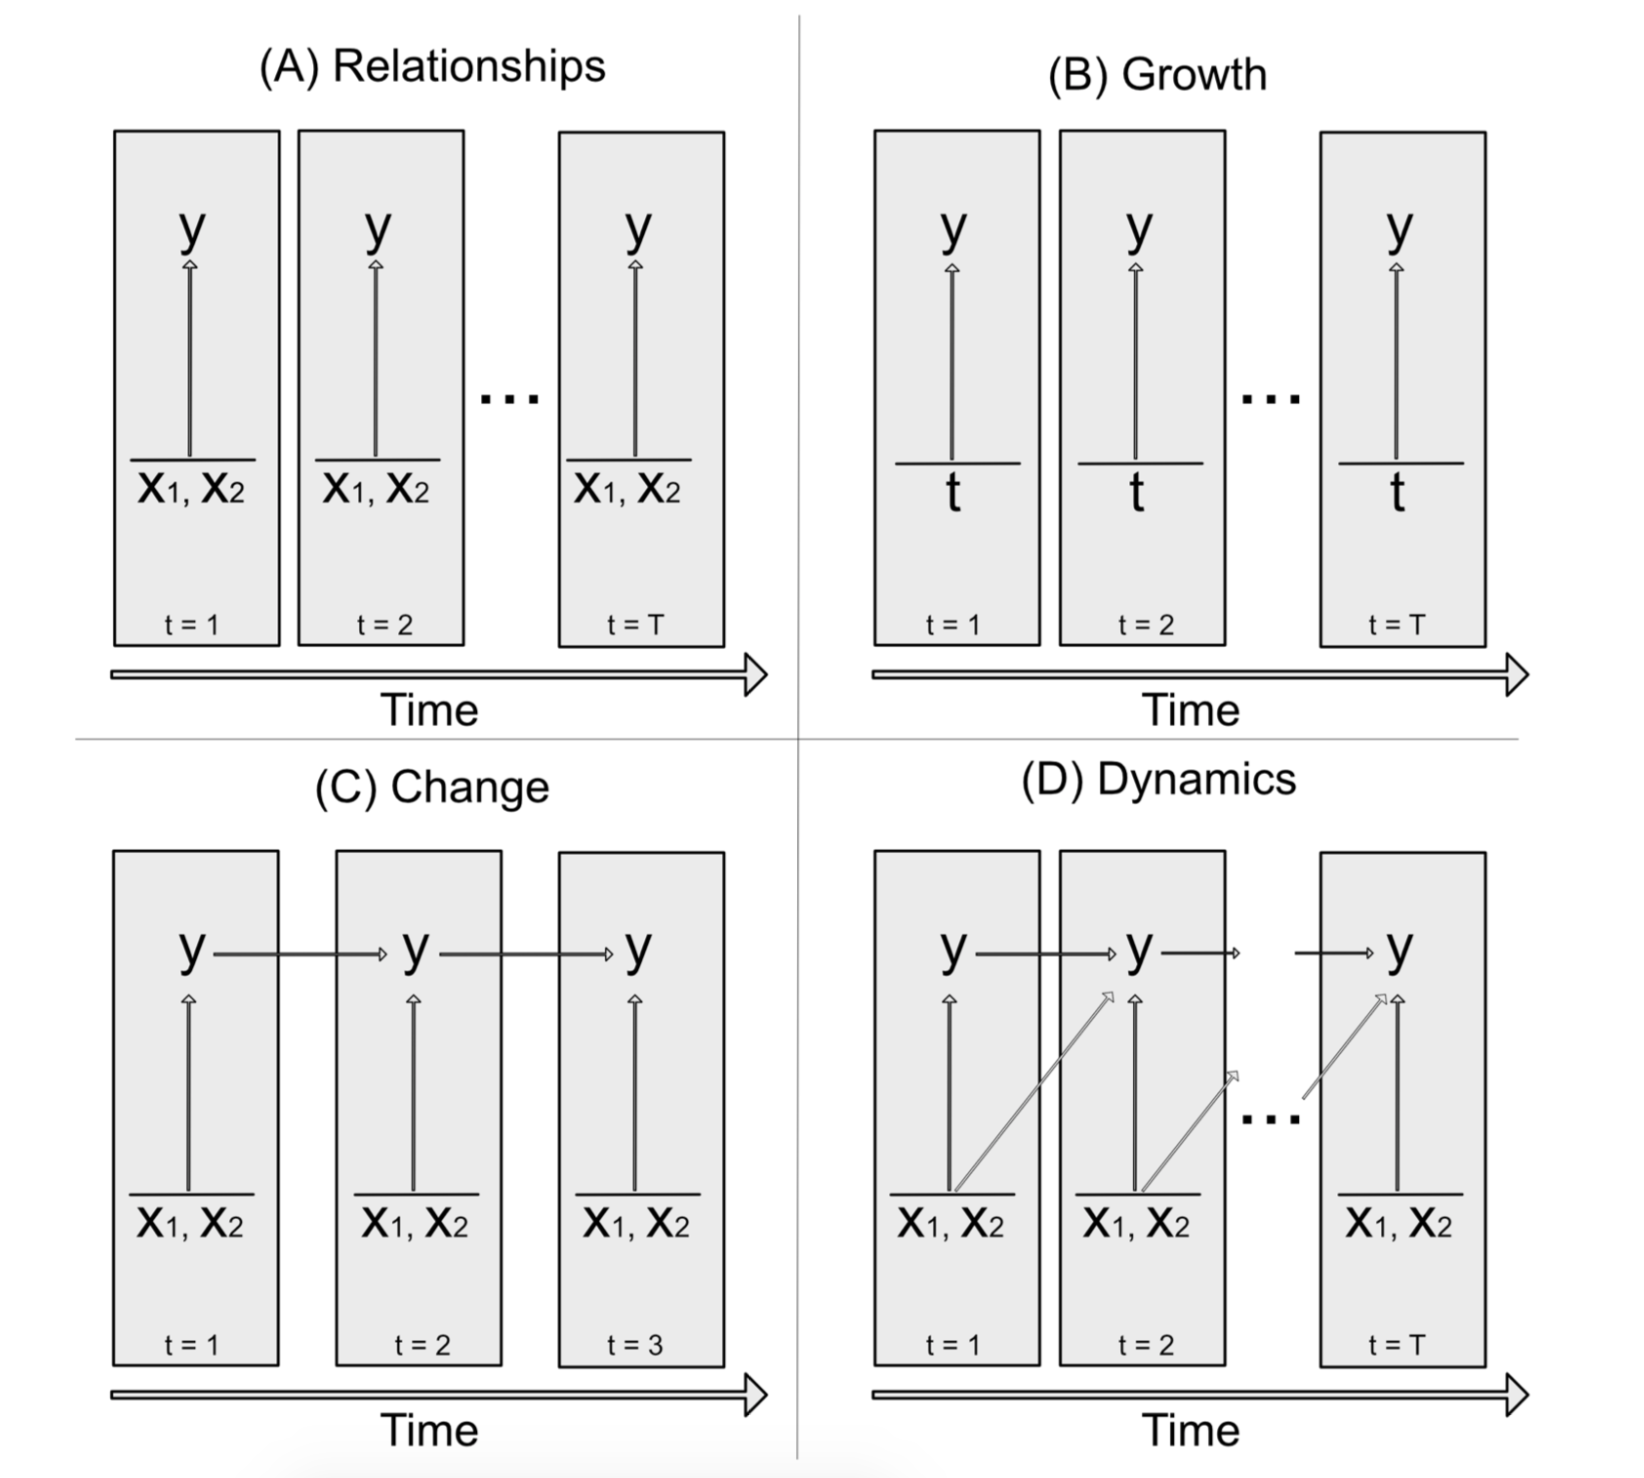
\includegraphics{figures/common_models.png}

\hypertarget{introduce-data-sets-and-generic-variables}{%
\subsection{Introduce data sets and generic
variables}\label{introduce-data-sets-and-generic-variables}}

We will use two generic variables -- affect (\(x\)) and performance
(\(y\)) -- throughout this paper. These variables will hopefully provide
continuity across the inferences and also provide an illuminating
backdrop after we refer to \(x\) or \(y\) generically. Moreover, we use
code examples in each section that refer to data sets that contain
measures of affect and performance on 50 simulated subjects across five
time points.

These data are contained in two data sets: \texttt{long\_df} and
\texttt{wide\_df}. The raw data are the same, but their formatting
differs because different estimation techniques require different data
structures. Structural equations modeling (SEM) requires wide data,
whereas HLM requires long data. The first data set, \texttt{long\_df}
contain the data in long form,

\begin{tabular}{r|r|r|r}
\hline
affect & performance & id & time\\
\hline
10.269606 & 17.23310 & 1 & 1\\
\hline
9.370015 & 22.81949 & 2 & 1\\
\hline
10.868660 & 17.64258 & 3 & 1\\
\hline
11.727196 & 20.56741 & 4 & 1\\
\hline
10.024188 & 12.08548 & 5 & 1\\
\hline
10.368025 & 13.17514 & 6 & 1\\
\hline
8.690796 & 12.76671 & 7 & 1\\
\hline
10.738622 & 13.62823 & 8 & 1\\
\hline
\end{tabular}

\noindent where \texttt{id} refers to a person identifier, \texttt{time}
refers to the observation period, and scores on \texttt{affect} and
\texttt{performance} are listed in their respective columns.

The second data set, \texttt{wide\_df} contain the data in wide form,

\begin{tabular}{r|r|r|r|r|r|r}
\hline
id & affect.1 & performance.1 & affect.2 & performance.2 & affect.3 & performance.3\\
\hline
1 & 10.269606 & 17.23310 & 9.945866 & 13.653924 & 9.059233 & 20.944278\\
\hline
2 & 9.370015 & 22.81949 & 10.461612 & 10.886965 & 10.093910 & 16.578068\\
\hline
3 & 10.868660 & 17.64258 & 9.403230 & 9.386411 & 10.066253 & 10.834513\\
\hline
4 & 11.727196 & 20.56741 & 11.263258 & 20.491540 & 9.009344 & 8.547953\\
\hline
5 & 10.024188 & 12.08548 & 8.854671 & 16.052982 & 9.927885 & 16.759775\\
\hline
6 & 10.368025 & 13.17514 & 11.084624 & 13.839404 & 9.776743 & 26.595386\\
\hline
7 & 8.690796 & 12.76671 & 8.471005 & 13.229533 & 9.857223 & 10.831559\\
\hline
8 & 10.738622 & 13.62823 & 8.426258 & 16.364850 & 10.535407 & 8.794605\\
\hline
\end{tabular}

\noindent where \texttt{id} is defined above and now \texttt{affect} and
\texttt{performance} are given new columns at each measurement period --
such that, as an example, person one reports 10.3 for affect at time one
and 9.9 for affect at time two (the data continue for five time points).
Again, we will refer to these variables and data sets as we unpack each
section, but remember that the values within each data set are the same
-- the only difference is their format.

\hypertarget{introduce-code-and-its-use}{%
\subsection{Introduce Code and Its
Use}\label{introduce-code-and-its-use}}

Finally, we will also present code snippets that estimate models related
to each inference. Code is typically published in methods literature to
demonstrate how to estimate models, but it can also be used as a tool --
a language -- to build a greater understanding of the phenomenon (nature
of code cite). We would like to use it for both reasons. Our goal is to
provide readers with code for estimating models, but also allow them to
see the inferences represented in various ways -- words and code -- to
help clarify what they represent.

The code snippets will take consistent forms throughout. HLM models will
be expressed as follows:

\begin{Shaded}
\begin{Highlighting}[]
\NormalTok{hlm_model <-}\StringTok{ }\KeywordTok{lme}\NormalTok{(}
  
\NormalTok{  code}
\NormalTok{  more code}
  
  \DataTypeTok{data =}\NormalTok{ long_df}
  
\NormalTok{)}
\end{Highlighting}
\end{Shaded}

\noindent where \texttt{hlm\_model} is an object that stores the results
of our model, \texttt{lme} is a function call to a linear mixed-effects
regression (HLM), and within that we specify our effects and reference
our data. In the inference sections, \texttt{code} and
\texttt{more\ code} will be replaced by the effects we estimate, and
\texttt{data} will always reference \texttt{long\_df} because HLM
requires long formatted data. Finally, after storing our results in the
object \texttt{hlm\_model} we can actually view them with:

\begin{Shaded}
\begin{Highlighting}[]
\KeywordTok{summary}\NormalTok{(hlm_model)}
\end{Highlighting}
\end{Shaded}

\noindent Similarly, SEM models will be expressed as:

\begin{Shaded}
\begin{Highlighting}[]
\NormalTok{sem_string <-}\StringTok{ '}

\StringTok{    code}
\StringTok{    more code}

\StringTok{'}

\NormalTok{sem_model <-}\StringTok{ }\KeywordTok{sem}\NormalTok{(sem_string, }
                 \DataTypeTok{data =}\NormalTok{ wide_df)}
\end{Highlighting}
\end{Shaded}

\noindent where \texttt{sem\_model} is an object that stores the results
of our SEM model and we refer to the \texttt{wide\_df} data set because
SEM requres wide data. Notice that in the SEM code snippet we first
create a string object, \texttt{sem\_string} to specify our effects.
Again, the \texttt{code} and \texttt{more\ code} will be replaced by
actual effects when we get to our inferences. Just like the HLM code, we
then view our SEM results with:

\begin{Shaded}
\begin{Highlighting}[]
\KeywordTok{summary}\NormalTok{(sem_model)}
\end{Highlighting}
\end{Shaded}

In summary, the style of code snippets just presented will be used
throughout each inference section. What will change are the
\texttt{code} and \texttt{more\ code} pieces, and in those areas we will
impute effects specific to each inference. If you wish to run these
models on your own computer, you will also need to load their packages
in your \texttt{r} script with \texttt{library(nlme)} for HLM and
\texttt{library(lavaan)} for SEM (and install them with
\texttt{install.packages()} if you have not done so already).

We now turn to the inferences.

\hypertarget{relationships}{%
\section{Relationships}\label{relationships}}

\hypertarget{inference-1}{%
\subsection{Inference 1}\label{inference-1}}

What is the relationship between two or more variables across time?

\hypertarget{explanation}{%
\subsection{Explanation}\label{explanation}}

A common inference in our longitudinal literature is the relationship
between an outcome (\(y\)) and one or more predictors (\(x_{p}\)) over
time. As shown in figure one, researchers observe \(y\) and one or more
predictors at each time point, and are then interested in the immediate
effect of the predictors on \(y\). Although there are multiple slices in
our figure, typically the effect of \(x\) on \(y\) is treated as stable
over time and therefore the analysis returns an estimate of a single
parameter (e.g., a single beta weight). This parameter is essentially a
summary statement of the immediate effect of \(x\) on \(y\) at any point
in time. In other words, researchers observe \(x\) and \(y\) at every
\(t\) from time \(t\) to \(t + 5\), as an example, and then report a
statement of the effect of \(x_{t}\) on \(y_{t}\), or the expected
immediate effect of \(x\) on \(y\) at any possible moment.

Although the effect (i.e., the parameter relating \(x\) to \(y\)) is
treated as stable over time, the values on \(x\) and \(y\) -- the raw
data -- are typically allowed to vary. When the values of \(x\)
(potentially) change at each observation, the analysis is referred to as
a time-varying covariates analysis -- whereas a time-invariant analysis
would be one where the raw data on \(x\) does not change at each
observation (e.g., gender).

To clarify, consider this inference with respect to our generic
variables: affect \(x\) and performance \(y\). Researchers would collect
performance and affect data on multiple people at each observation over
several time points. Affect may vary at each observation -- it may be 5
at time \(t\) and 9 at time \(t + 1\) -- so this analysis is referred to
as a time-varying covariates analysis. Researchers are then interested
in the stable, immediate influence of affect on performance. That is,
they are interested in the effect of affect\(_{t}\) on
performance\(_{t}\) at any potential \(t\), where, on average, they
expect the effect of affect on performance to be close to their
parameter value.

There is a distinction with how we use the term \enquote{stable} that
merits more explanation. In a relationships inference, \enquote{stable}
means that we expect the parameter value relating affect to performance
to be the same at each moment. In other words, the relationship between
affect and performance will be the same at each \(t\) -- high values of
affect will result in high values of performance (if the parameter is
positive) and low values of affect will result in low values of
performance. \enquote{Stable} in this inference context does not mean
that affect has a lasting impression on performance, or that affect at
time \(t\) influences performance at some later time. This distinction
is a difficult one, but it represents a major difference betweeen making
a relationships inference versus some of the others we have yet to
explore. A relationships inference, therefore, is concerned with the
average influence over time, or what we expect the immediate effect of
\(x\) on \(y\) to be at any given moment.

\hypertarget{literature-examples-and-hypotheses}{%
\subsection{Literature Examples and
Hypotheses}\label{literature-examples-and-hypotheses}}

There are many examples in our literature that are interested in
relationships over time. When a researcher is interested in making a
relationships inference, they propose a hypothesis of the form: \(x\)
predicts \(y\) (given some direction, positive or negative). Using our
generic variables, we would propose:

\hypertarget{affect-positively-or-negatively-predicts-performance-over-time.}{%
\paragraph{Affect positively (or negatively) predicts performance over
time.}\label{affect-positively-or-negatively-predicts-performance-over-time.}}

\noindent For example, Barnes, Schaubroeck, Huth, and Ghumman (2011)
predict a negative relationship between poor sleep and cognitive self
control. Similarly, Chi, Chang, and Huang (2015) hypothesize that daily
negative mood negatively relates to daily task performance.

\hypertarget{code}{%
\subsection{Code}\label{code}}

We gain even more clarity on this inference when we consider the code
used to estimate models. A typical SEM model would be estimated with
something similar to the following code.

\begin{Shaded}
\begin{Highlighting}[]
\NormalTok{sem_string <-}\StringTok{ '}

\StringTok{      performance.1 ~ b1*affect.1}
\StringTok{      performance.2 ~ b1*affect.2}
\StringTok{      performance.3 ~ b1*affect.3}
\StringTok{      performance.4 ~ b1*affect.4}
\StringTok{      performance.5 ~ b1*affect.5}

\StringTok{'}
\KeywordTok{sem}\NormalTok{(sem_string, }\DataTypeTok{data =}\NormalTok{ wide_df)}
\end{Highlighting}
\end{Shaded}

\noindent where this code snippet is identical to our introductory SEM
code but we have replaced \texttt{code} and \texttt{more\ code} with
actual effects we wish to estimate. In this case, we regress performance
at time \(t\) on affect at time \(t\) and estimate \texttt{b1} -- the
parameter relating affect to performance over time. The analysis will
return one number for \texttt{b1} because, again, we are treating this
as a stable estimate over time.

The HLM equivalent would be:

\begin{Shaded}
\begin{Highlighting}[]
\KeywordTok{lme}\NormalTok{(                                   }
  
  \DataTypeTok{fixed =}\NormalTok{ performance }\OperatorTok{~}\StringTok{ }\NormalTok{affect,}
  \DataTypeTok{random =} \OperatorTok{~}\DecValTok{1}\OperatorTok{|}\NormalTok{id,}
  \DataTypeTok{data =}\NormalTok{ long_df}
  
\NormalTok{)}
\end{Highlighting}
\end{Shaded}

\noindent where we again replace \texttt{code} and \texttt{more\ code}
from the introductory HLM snippet with a regression of performance on
affect. Notice that we do not need to type the performance on affect
regressions at each time point as we did with the SEM code. Typically,
in SEM software you type out the entire model, whereas HLM packages use
condensed code. There are two other new pieces of code: \texttt{fixed}
and \texttt{random}. These commands specify how we want HLM to estimate
the parameters we are interested in, but at this point we do not unpack
them further -- we will return to what they mean in the full modeling
section at the end of the paper.

We will devote an entire section to the statistical properties of HLM
and SEM below, what is important here is our regression of performance
on affect. In both HLM and SEM we estimate a stable parameter relating
affect at time \(t\) to performance at time \(t\) -- in SEM software we
explicitly identify a parameter (\texttt{b1}) whereas HLM software
typically does so automatically.

\hypertarget{relationships-inference-1-summary}{%
\subsection{Relationships Inference 1
Summary}\label{relationships-inference-1-summary}}

\begin{itemize}
\item
  Hypothesis:

  \begin{itemize}
  \tightlist
  \item
    \(x\) relates to \(y\) over time.
  \end{itemize}
\item
  Parameters From SEM or HLM:

  \begin{itemize}
  \tightlist
  \item
    beta coefficient relating \(x\) to \(y\) at each time point.
  \end{itemize}
\end{itemize}

\hypertarget{growth}{%
\section{Growth}\label{growth}}

We now move to our second inference panel, \(B\) and explore a variety
of inferences related to growth.

\hypertarget{inference-1-1}{%
\subsection{Inference 1}\label{inference-1-1}}

What is the level of a construct at a given point in time?

\newpage

\hypertarget{references}{%
\section{References}\label{references}}

\setlength{\parindent}{-0.5in}
\setlength{\leftskip}{0.5in}

\hypertarget{refs}{}
\leavevmode\hypertarget{ref-barnes2011}{}%
Barnes, C. M., Schaubroeck, J., Huth, M., \& Ghumman, S. (2011). Lack of
sleep and unethical conduct. \emph{Organizational Behavior and Human
Decision Processes}, \emph{115}(2), 169--180.

\leavevmode\hypertarget{ref-chi2015}{}%
Chi, N.-W., Chang, H.-T., \& Huang, H.-L. (2015). Can personality traits
and daily positive mood buffer the harmful effects of daily negative
mood on task performance and service sabotage? A self-control
perspective. \emph{Organizational Behavior and Human Decision
Processes}, \emph{131}, 1--15.

\leavevmode\hypertarget{ref-gabriel2014}{}%
Gabriel, A. S., Diefendorff, J. M., Chandler, M. M., Moran, C. M., \&
Greguras, G. J. (2014). The dynamic relationships of work affect and job
satisfaction with perceptions of fit. \emph{Personnel Psychology},
\emph{67}(2), 389--420.

\leavevmode\hypertarget{ref-hardy2018}{}%
Hardy, J. H., Day, E. A., \& Steele, L. M. (2018). Interrelationships
among self-regulated learning processes: Toward a dynamic process-based
model of self-regulated learning. \emph{Journal of Management},
0149206318780440.

\leavevmode\hypertarget{ref-johnson2014}{}%
Johnson, R. E., Lanaj, K., \& Barnes, C. M. (2014). The good and bad of
being fair: Effects of procedural and interpersonal justice behaviors on
regulatory resources. \emph{Journal of Applied Psychology},
\emph{99}(4), 635.

\leavevmode\hypertarget{ref-jones2016}{}%
Jones, K. P., King, E. B., Gilrane, V. L., McCausland, T. C., Cortina,
J. M., \& Grimm, K. J. (2016). The baby bump: Managing a dynamic stigma
over time. \emph{Journal of Management}, \emph{42}(6), 1530--1556.

\leavevmode\hypertarget{ref-matthews2014}{}%
Matthews, R. A., Wayne, J. H., \& Ford, M. T. (2014). A work--family
conflict/subjective well-being process model: A test of competing
theories of longitudinal effects. \emph{Journal of Applied Psychology},
\emph{99}(6), 1173.

\leavevmode\hypertarget{ref-meier2013}{}%
Meier, L. L., \& Spector, P. E. (2013). Reciprocal effects of work
stressors and counterproductive work behavior: A five-wave longitudinal
study. \emph{Journal of Applied Psychology}, \emph{98}(3), 529.

\leavevmode\hypertarget{ref-rosen2016}{}%
Rosen, C. C., Koopman, J., Gabriel, A. S., \& Johnson, R. E. (2016). Who
strikes back? A daily investigation of when and why incivility begets
incivility. \emph{Journal of Applied Psychology}, \emph{101}(11), 1620.


\end{document}
